
\section{Methodology}


\subsection{Model Architecture}

\begin{enumerate}
			\item Embedding Layer
			\item Bidirectional LSTM Layer
			\item Linear Layer
\end{enumerate}

\begin{figure}[h]
	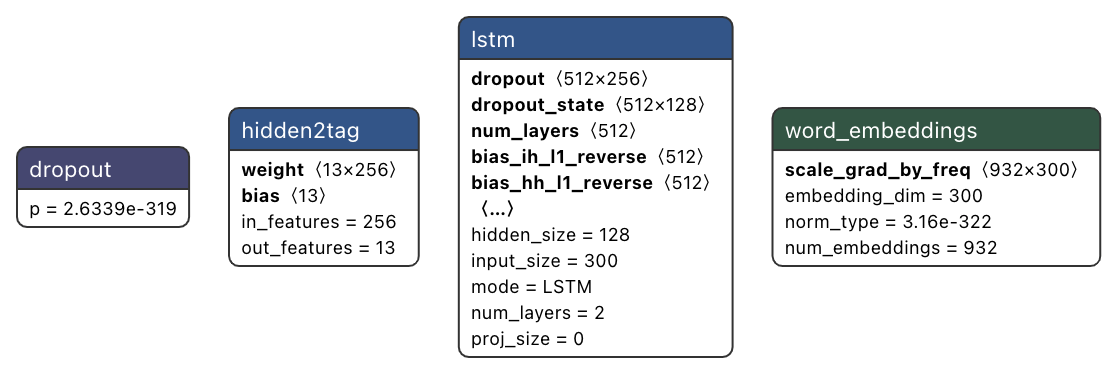
\includegraphics[scale=0.4]{img/model_arch.png}
	\caption{Model Architecture}
\end{figure}

\begin{itemize}
	\item I have used Bidirectional LSTM in POS tagging of English language because in English language, the POS tag of a word can depend on the words that come before and after it. By using a bidirectional LSTM, we can take into account both the preceding and following words when predicting the POS tag for a particular word. This helps to capture the context of the sentence better and leads to more accurate POS tagging.
	\item I have incorporated Dropout in the model since the corpus being used is small, which increases the risk of overfitting. By dropping some of the weights and re-learning them in subsequent iterations, the model can prevent overfitting.
\end{itemize}


\subsection{Implementational Steps}

Steps followed to implement the Neural POS Tagger

\begin{enumerate}
	\item Examine the dataset to understand the available data and its structure in detail.
	\item Created sequence of the dataset in order to feed the model
	\begin{lstlisting}[language=Python]
	def prepare_datasets(dataset):
    	mod_data = []
   		for idx in range(len(dataset)):
       		tempword = []
       		temptag = []
       		for jdx in range(len(dataset[idx])):
           		tempword.append(dataset[idx][jdx]["form"])
           		temptag.append(dataset[idx][jdx]["upos"])

        	mod_data.append([tempword, temptag])
    	return mod_data
	\end{lstlisting}
	
	\item Create vocabulary for Train Dataset (both for word tokens as well as Tag Tokens), for this I have used \texttt{torchtext vocabulary builder}, which lets us created a dictionary which handles the unknowns.
	\begin{lstlisting}[language=Python]
	word_vocab = torchtext.vocab.build_vocab_from_iterator(new_list)
	word_vocab.insert_token('<unk>', 0)            
	word_vocab.set_default_index(word_vocab['<unk>'])
	\end{lstlisting}

	\item Create model, \texttt{pytorch} let's you create model using class inheritence. I have used 3 layers to define my model as defined in Model Architecture.
	
	\begin{lstlisting}[language=Python]
	class LSTMTagger(nn.Module):
    	def __init__(
        	self,
        	word_embedding_dim,
        	word_hidden_dim,
        	vocab_size,
        	tagset_size,
    	):
        	super(LSTMTagger, self).__init__()
        	self.word_hidden_dim = word_hidden_dim
        	self.word_embeddings = nn.Embedding(vocab_size, word_embedding_dim)
        	self.lstm = nn.LSTM(word_embedding_dim, word_hidden_dim, num_layers = 1, bidirectional = True)

        	self.hidden2tag = nn.Linear(word_hidden_dim*2, tagset_size)

        	self.dropout = nn.Dropout(0.1)

    	def forward(self, sentence):
        	embeds = self.dropout(self.word_embeddings(sentence))
        	lstm_out, _ = self.lstm(embeds.view(len(sentence), 1, -1))
        	tag_space = self.hidden2tag(lstm_out.view(len(sentence), -1))
        	tag_scores = F.log_softmax(tag_space, dim=1)
        	return tag_scores

	\end{lstlisting}
	
	\item To optimise the model during training, I have used the \textit{cross entropy loss function} and the \textit{Adam optimiser} to update the model's parameters based on the gradients calculated during back-propagation. The \textit{cross entropy} loss function is used because it is commonly used for multi-class classification tasks. The Adam optimiser is a popular optimisation algorithm that adapts the learning rate during training to improve convergence.

	\begin{lstlisting}[language=Python]
	loss_function = nn.CrossEntropyLoss()
	optimiser = optim.Adam(model.parameters(), lr=LEARNING_RATE)
	\end{lstlisting}

	\item I have experimented with different values of \textit{hyper-parameters} and have decided on some based on my observations. I noticed that the model performed better with smaller values for the embedding size and hidden layer, which may be due to the small size of the corpus. The following are the finalised \textit{hyper-parameters}

	\begin{lstlisting}[language=Python]
	WORD_EMBEDDING_DIM = 64
	WORD_HIDDEN_DIM = 64
	EPOCHS = 50
	BIDIRECTIONAL = True
	DROPOUT = 0.5
	LEARNING_RATE = 0.005
	\end{lstlisting}
	
	
	
	
	
	
	
\end{enumerate}